\documentclass[a4paper,10pt]{article}
\usepackage[margin=1in]{geometry}
\usepackage{polski}
\usepackage[utf8x]{inputenc}
\usepackage[unicode]{hyperref}
\usepackage{amssymb}
\usepackage{xifthen}
\usepackage[fleqn]{amsmath}
\usepackage{todonotes}
\usepackage{graphicx}
\usepackage{float}
\usepackage{fullpage}
\usepackage{epstopdf}
\usepackage{multirow}
\usepackage{subfig}
\usepackage{booktabs}
\usepackage[europeanresistors,americaninductors]{circuitikz}
\usetikzlibrary{patterns}
\newcommand{\withtodo}{0}

\def\arraystretch{1.2}

\begin{document}

\begin{table}
  \centering
  \def\arraystretch{1.5}
    \begin{tabular}{|l|l|l|l|} \hline
    Wydział:           & \multicolumn{2}{l|}{Dzień:Poniedziałek 14-17}    &Zespół:  \\
    Fizyki             &    \multicolumn{2}{l|}{Data: 20.03.2017}         &8             \\\hline
    Imiona i nazwiska: &Ocena z przygotowania:  &Ocena ze sprawozdania:   &Ocena końcowa: \\
    Marta Pogorzelska  &                        &                         &                \\
    Paulina Marikin    &                        &                         &\\\hline
    \multicolumn{2}{|l|}{Prowadzący:                 } &\multicolumn{2}{l|}{Podpis:             }  \\\hline
  \end{tabular}
\end{table}

\title{Ćwiczenie 20:\\Badanie właściwości magnetycznych ciał stałych}
\date{}
\maketitle{}

\section{Cel badań}
Zapoznanie się z właściwościami magnetycznymi ciał stałych oraz wyznaczenie temperatury Curie dla rdzenia ferromagnetycznego w transformatorze.

\section{Wstęp teoretyczny}
Magnetyzm jest to zjawisko i właściwości fizyczne materii związane z oddziaływaniem ciał poprzez pole magnetyczne. Jego źródłem mogą być naładowane ciała, np.:
magnes, pojedyncze cząsteczki lub przewodniki z prądem. Ze względu na sposób oddziaływania danego ciała na zewnętrzne pole magnetyczne można podzielić je na:
ferromagnetyki, paramagnetyki, diamagnetyki, anty-ferromagnetyki oraz ferrimagnetyki. Jednostką opisującą stopień w jakim dane ciało wykazuje zdolności magnetyczne
jest magnetyzacja lub namagnesowanie - $\vec{M}$. Wyraża się ona wzorem:
\begin{equation}
\vec{M} =\frac{1}{V} \sum_{i=1}^n \vec{\mu_i}
\end{equation}
,gdzie V – objętość, $\vec{\mu_i}$ - elementarny moment magnetyczny.
\\%W tym akapicie 2 wykresy teoretyczne
\\Zarówno ferromagnetyki i paramagnetyki posiadają niezerowy moment magnetyczny, ale  tylko ferromagnetyki charakteryzują się istnieniem wewnętrznego pola
magnetycznego porządkującego spiny, co objawia się niezerowym namagnesowaniem jego próbek. Podczas gdy spiny paramagnetyków niezależnie od temperatur pozostają
nieuporządkowane a ich kierunki są całkowicie przypadkowe. Wraz ze wzrostem temperatury ferrromagnetyka, wzrastają chaotyczne fluktuacje spinów. Temperatura w której fluktuacje całkowicie niszczą wewnętrzne domeny magnetyczne, zaś ferromagnetyk przechodzi do fazy paramagnetycznej jest nazywana temperaturą Curie. Jest to przejście fazowe drugiego rodzaju.
\paragraph{Wykresy teoretyczne magnetyzacji ferromagnetyka}
%\begin{figure}[H]
%		\includegraphics[width=0.4\textwidth]{droga/dostępu.png}
%		\caption{przy braku pola zewnętrznego}
%\end{figure}
%\begin{figure}[H]
%		\includegraphics[width=0.4\textwidth]{droga/dostępu.png}
%		\caption{w niezerowym zewnętrznym polu magnetycznym}
%\end{figure}
W celu uporządkowania układu momentów magnetycznych ferromagnetyka w fazie paramagnetycznej można
przyłożyć wystarczająco silne zewnętrzne pole magnetyczne albo obniżyć temperaturę danej próbki. Skutkuje to ponownym powstaniem coraz większych wraz ze zmniejszeniem temperatury domen magnetycznych.
\\
\\Jak wspomniano wyżej, jednym ze sposobów na uporządkowanie układu spinów jest przyłożenie zewnętrznego pola magnetycznego. Wielkością charakteryzującą jego reakcję
na takie pole jest podatność magnetyczna i wyraża się ona wzorem:
\begin{equation}
\chi = \frac{M}{H}
\end{equation}
,gdzie H - natężenie pola magnetycznego.
\end{equation}
\\
\\Prawo Curie-Weissa, opisujące zachowanie ferromagnetyków w $T > \theta$,mówi:
\begin{equation}
\chi = \frac{C}{T - \theta}
\end{equation}
,gdzie C - stała Curie-Weissa, T - temperatura próbki, $\theta$ - temperatura Curie-Weissa.
\\
\\Napięcie wtórne na transformatorze, które będzie mierzone w tym doświadczeniu jest liniowo zależne od i indukcyjności:
\begin{equation}
U = U_0 + AM(T)
\end{equation}
gdzie A to dowolna stała. W celu wyznaczenia $\theta$ przekształcamy wzór (3) i otrzymujemy:
\begin{equation}
\frac{1}{\chi} = \frac{1}{C} T - \frac{\theta}{C} = \frac{1}{C} (T-\theta)
\end{equation}
Przedstawiona zależność odwrotności podatności od temperatury jest zależnością liniową.

\section{Opis układu i metody pomiarowej}
Doświadczenie polegało na wyznaczeniu, za pomocą serii pomiarów napięcia na uzwojeniu wtórnym transformatora w zależności od temperatury, temperatury Curie dla
ferromagnetycznego rdzenia tego transformatora. Po włączeniu komputera i specjalnego programu należało rozgrzać grzałkę najpierw do 20\% jej mocy i odnotować
kilka pomiarów napięcia dla danej temperatury. Następnie ustawiono moc grzałki na 70\%, odnotowano kilka pomiarów dla nowej temperatury, a następnie pozostawiono
układ na ok 1,5 godziny w celu osiągnięcia przez grzałkę oczekiwanej temperatury. Po upływie czasu dokonywano pomiarów co minutę, za każdym razem podwyższając moc grzałki o 1\% i powtarzając czynność aż moc wyniesie 100\%. Na koniec obniżono moc grzałki w celu wychłodzenia układu i po odczekaniu chwili wyłączono komputer oraz odłączono układ od prądu.
\begin{figure}[H]
\center
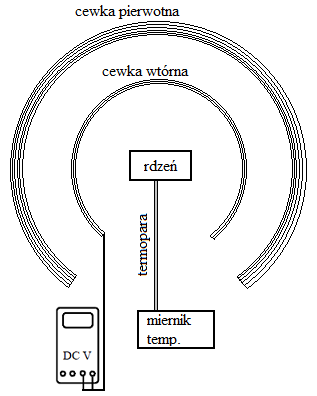
\includegraphics[width=0.4\textwidth]{uklad.png}
\end{figure}
Na przedstawiony powyżej układ użyty w doświadczeniu składa się: źródło prądu zmiennego, uzwojenie pierwotne transformatora $n_p$, uzwojenie wtórne transformatora $n_w$, ferromagnetyczny rdzeń, termometr elektroniczny podłączony do próbki, woltomierz cyfrowy oraz grzałka. Całość układu podłączona jest do komputera ze specjalnym oprogramowaniem, dzięki któremu można zmieniać moc grzałki oraz który archiwizuje otrzymane wyniki i nanosi je na wykres zależności napięcia od temperatury.

\section{Wyniki i analiza pomiarów}
\subsection{Wyznaczanie temperatury Curie}
Tabela danych pomiarowych wraz z niepewnościami.
\begin{figure}[H]
\begin{tabular}{lrrrr}
\hline
{} &T[$^\circ$C]&$\Delta T[^\circ$C]&U[mV]&$\Delta$ U[mV]\\
\hline
  &   20.0 &  5.1 &  452 &  11 \\
  &   95.0 &  5.4 &  452 &  11 \\
  &  117.0 &  5.5 &  449 &  11 \\
  &  122.0 &  5.6 &  447 &  11 \\
  &  128.0 &  5.6 &  442 &  11 \\
  &  133.0 &  5.6 &  436 &  11 \\
  &  137.0 &  5.6 &  435 &  11 \\
  &  141.0 &  5.7 &  429 &  11 \\
  &  144.0 &  5.7 &  422 &  11 \\
  &  147.0 &  5.7 &  416 &  11 \\
 &  150.0 &  5.7 &  407 &  11 \\
 &  153.0 &  5.7 &  396 &  10 \\
 &  156.0 &  5.7 &  383 &  10 \\
 &  159.0 &  5.7 &  361 &  10 \\
 &  162.0 &  5.8 &  334 &  10 \\
 &  165.0 &  5.8 &  301.0 &   9.5 \\
 &  168.0 &  5.8 &  262.0 &   8.9 \\
 &  170.0 &  5.8 &  221.0 &   8.3 \\
 &  173.0 &  5.8 &  183.0 &   7.7 \\
 &  176.0 &  5.8 &  146.0 &   7.1 \\
 &  179.0 &  5.8 &  111.0 &   6.6 \\
 &  183.0 &  5.9 &   78.0 &   6.1 \\
 &  186.0 &  5.9 &   57.0 &   5.8 \\
 &  189.0 &  5.9 &   42.0 &   5.6 \\
 &  192.0 &  5.9 &   34.0 &   5.5 \\
 &  195.0 &  5.9 &   29.0 &   5.4 \\
 &  198.0 &  5.9 &   25.0 &   5.3 \\
 &  201.0 &  6.0 &   22.0 &   5.3 \\
 &  203.0 &  6.0 &   21.0 &   5.3 \\
 &  206.0 &  6.0 &   20.0 &   5.3 \\
 &  208.0 &  6.0 &   19.0 &   5.2 \\
 &  211.0 &  6.0 &   18.0 &   5.2 \\
\hline
\end{tabular}
\end{figure}
W celu wyznaczenia temperatury Curie powyższe pomiary zostały przedstawione na rysunku 3:
\begin{figure}[H]
  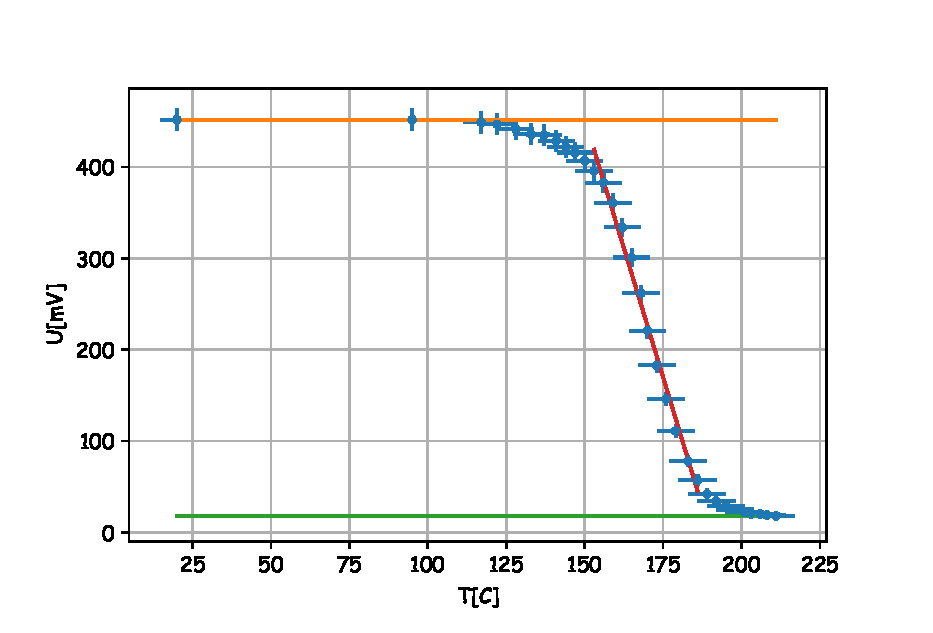
\includegraphics{./Curie_proste.eps}
  \caption{Wykres zależności $U(T)$ z prostymi dla maksymalnego i minimalnego napięcia oraz prostą dopasowaną do najostrzejszej części wykresu}
\end{figure}.
%Nie wiem czy coś jeszcze dopisać, chyba jest git
\\Na wykresie 1 wartości napięcia utrzymują mniej-więcej(w zakresie błędów pomiarowych) stały poziom dla temperatur poniżej 128$^\circ$C (452mV -
wynikający z maksymalnego namagnesowania rdzenia)i temperatur powyżej 201$^\circ$C (18mV). Prosta dopasowana do pomiarów z najwyższym spadkiem leży najpierw
poniżej, a następnie powyżej punktów pomiarowych i przechodzi przez nie w temperaturze $T = 170^\circ C$, którą w związku z tym możemy uznać za temperature Curie. Jakościowy kształt wykresu czyli stały-łagodny_spadek-szybki_spadek-łagodny_spadek-stały odpowiada teoretycznemu rysunkowi 2 i tym samym potwierdza teorię.
\subsection{Wyznaczanie temperatury Curie-Weissa}
Aby sprawdzić prawdziwość prawa Curie-Weissa oraz w celu wyznaczenia temperatury $\theta$ pomiary przekształcono na sposób zaprezentowany w poniższej tabeli oraz przedstawiono na wykresach, które, zgodnie z prawem Curie-Weisa, powinny przedstawiać zależność liniową.
\begin{figure}
\begin{tabular}{lrrrrrr}
\toprule
{} &  T[$^\circ $C] &  $\Delta T [^\circ C]$ &  $\frac{1}{U}[\frac{1}{mV}]*10^{-4}$ &  $\Delta \frac{1}{U}[\frac{1}{mV}]$ &  $\frac{1}{U-U_{min}}[\frac{1}{mV}]$ &  $\Delta \frac{1}{U-U_{min}}[\frac{1}{mV}]$ \\
\midrule
& 170.0 &  5.8 & 221 & 1.7 & 0.005 &   2.0e-04 \\
& 173.0 &  5.8 & 183 & 2.3 & 0.006 &   2.8e-04 \\
& 176.0 &  5.8 & 146 & 3.3 & 0.008 &   4.3e-04 \\
& 179.0 &  5.8 & 111 & 5.4 & 0.011 &   7.7e-04 \\
& 183.0 &  5.9 &  78 & 10  & 0.017 &   1.7e-03 \\
& 186.0 &  5.9 &  57 & 18  & 0.026 &   3.8e-03 \\
& 189.0 &  5.9 &  42 & 31  & 0.042 &   9.7e-03 \\
& 192.0 &  5.9 &  34 & 47  & 0.062 &   2.1e-02 \\
& 195.0 &  5.9 &  29 & 64  & 0.091 &   4.4e-02 \\
& 198.0 &  5.9 &  25 & 86  & 0.143 &   1.0e-01 \\
& 201.0 &  6.0 &  22 & 110 & 0.250 &   3.3e-01 \\
& 203.0 &  6.0 &  21 & 120 & 0.333 &   5.9e-01 \\
& 206.0 &  6.0 &  20 & 130 & 0.500 &   1.3e+00 \\
& 208.0 &  6.0 &  19 & 140 & 1.000 &   5.2e+00 \\
& 211.0 &  6.0 &  18 & 160 &   inf &       inf \\
\bottomrule
\end{tabular}
\end{figure}
Niepewności przekształconych wartości zostały wyliczone z metody propagacji niepewności:
\begin{equation}
\Delta \frac{1}{U} = \frac{\Delta U}{U^2}
\end{equation}
\begin{figure}[H]
  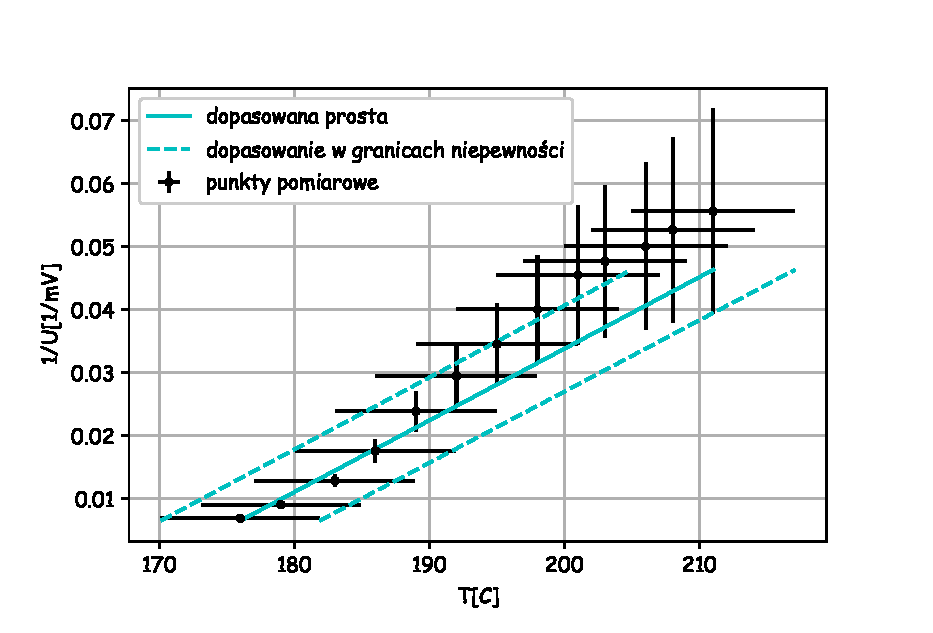
\includegraphics{./Curie_odwrotnosc.eps}
  \caption{Wykres zależności $\frac{1}{U}$(T) dla fazy paramagnetyka}
\end{figure}
\begin{figure}[H]
  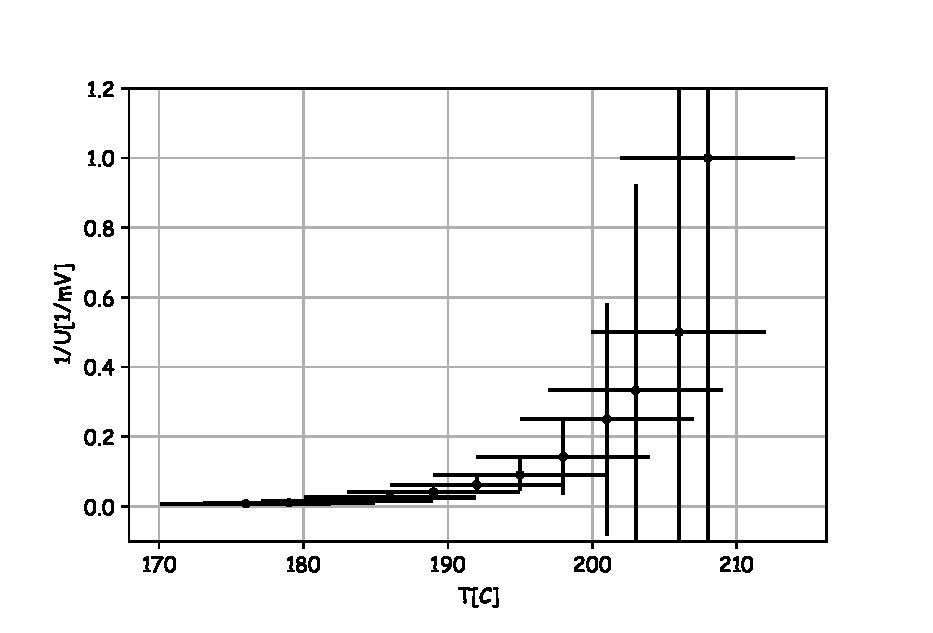
\includegraphics{./Curie_odjete.eps}
  \caption{Wykres zależności $\frac{1}{U-U_{min}}$(T) dla fazy paramagnetyka}
\end{figure}
\\Wykres 4 jest zgodnie z założeniami, liniowy. Wraz ze spadkiem napięcia rosną jego niepewności, a co za tym idzie kolejne punkty pomiarowe są coraz bardziej wątpliwe. W końcowej części wykresu powinno następować wypłaszczenie (Całkowite wzbudzenie przez uzwojenie wtórne) jednak jest ono niewidoczne. Może to być spowodowane sporymi niepewnościami w tym obszarze lub wciąż zbyt niskimi temperaturami. Dla dopasowanej prostej widać przesunięcie $\theta$ względem $T_C$ o około $5^\circ$. Do wykresu 4 dopasowano prostą przy użyciu funkcji \emph{polyfit}, biblioteki \emph{numpy} w Pytonie, z
użyciem wag $\frac{1}{dy}$. Dla wykresu 5 $U_{min}$ zostało oszacowane jako najmniejsza zmierzona wartość niapięcia. Jednak wykres ten jest, ze względu na szybko rosnące różnice i ogromne niepewności, nieczytelny i nie został poddany analizie. 
\\

\section{Analiza niepewności}
Niepewności pomiarów temperatury została wyliczona jako iloczyn danego pomiaru i klasy urządzenia pomiarowego(0.005) + 5$^\circ$C
Niepewności napięcia wyliczono tożsamą metodą dla klasy 0.01 i dodając 1mV.Metody użyte w analizie wyników nie były ściśle analityczne, co nie pozwala na bezpośrednie wyliczenie niepewności jednak można ją oszacować jako przedział maksymalnego spadku na $18c^\circ$.

\section{Wnioski}
Wykres (2) jest jakościowo zgodny z teoretycznym. Wyznaczona temperatura Curie wynosi $170(18)C^\circ$, jednak biorąc pod uwagę niepewność temperatury Curie, metoda, której użyto w tym doświadczeniu jest niezbyt niedokładna i nie nadaje się do jej wyznaczenia w celach praktycznych. Zależności wyliczone na podstawie wzoru (4) i przedstawione na wykresie (4) zdają się potwierdzać prawdziwość prawa Curie-Weissa .Wykres (5) nie nadaje się do analizy ze względu na zbyt duże niepewności i nie pozwala na potwierdzenie bądź odrzucenie tezy.


\end{document}
